\documentclass[a4paper,11pt]{article}
\usepackage{graphicx}
\usepackage[margin=2cm]{geometry}

\begin{document}
\title{Obligatorisk oppgave 7: Elektrodynamikk}
\author{Michael R. Johansen}
\date{November 3, 2023}
\maketitle

\newpage
\section*{Oppgave 11}
\raggedright

Konstanter oppgitt:

$$\Delta V = 1.2 \times 10^9\, \mathrm{V}$$
$$q = 25\, \mathrm{C}$$
$$m_{bil} = 1100\, \mathrm{Kg}$$

\section*{a)}

For å finne arbeidet gjort på partikkelen bruker vi formelen for arbeid gjort i et elektrisk felt:

$$W_{ab} = -q_0 \Delta V$$

Setter inn verdiene

$$W_{ab} =  25\, \mathrm{C} \times 1.2 \times 10^9\, \mathrm{V}$$

\centerline{\underline{\underline{$W_{ab} = 3.0 \times 10^{10}\, \mathrm{J}$}}}

\section*{b)}

Vi lar all abeidet gjort på partikkelen bli omgjort til kinetisk energi, vi antar også at resultantfarten ikke vil være relitavistisk. Uttrykket for fart er da: 
$$W_{ab} = \frac{1}{2}mv^2$$

Løser for farten

$$v = \sqrt{\frac{2W_{ab}}{m_{bil}}}$$

Setter inn verdiene:

$$v = \sqrt{\frac{2 \times  3.0 \times 10^{10}\, \mathrm{J}}{ 1100\, \mathrm{Kg}}}$$

\centerline{\underline{\underline{$v = 7.4 \times 10^{3}\, \mathrm{m/s}$}}}

\newpage
\section*{Oppgave 17}

\begin{minipage}{0.45\textwidth}
  % Your text goes here on the left side.
Ettersom vi ønsker å finne det totale potensialet i punktet P, kan vi benytte \textit{superposisjonsprinsippet} til å finne resultantpotensialet fra de fire punktladningene.

Konstanter:

$$d = 0.96\, \mathrm{m}$$
$$q = 2.0 \mu \, \mathrm{C}$$

\end{minipage}%
\begin{minipage}{0.55\textwidth}
  % Your image goes here on the right side.
  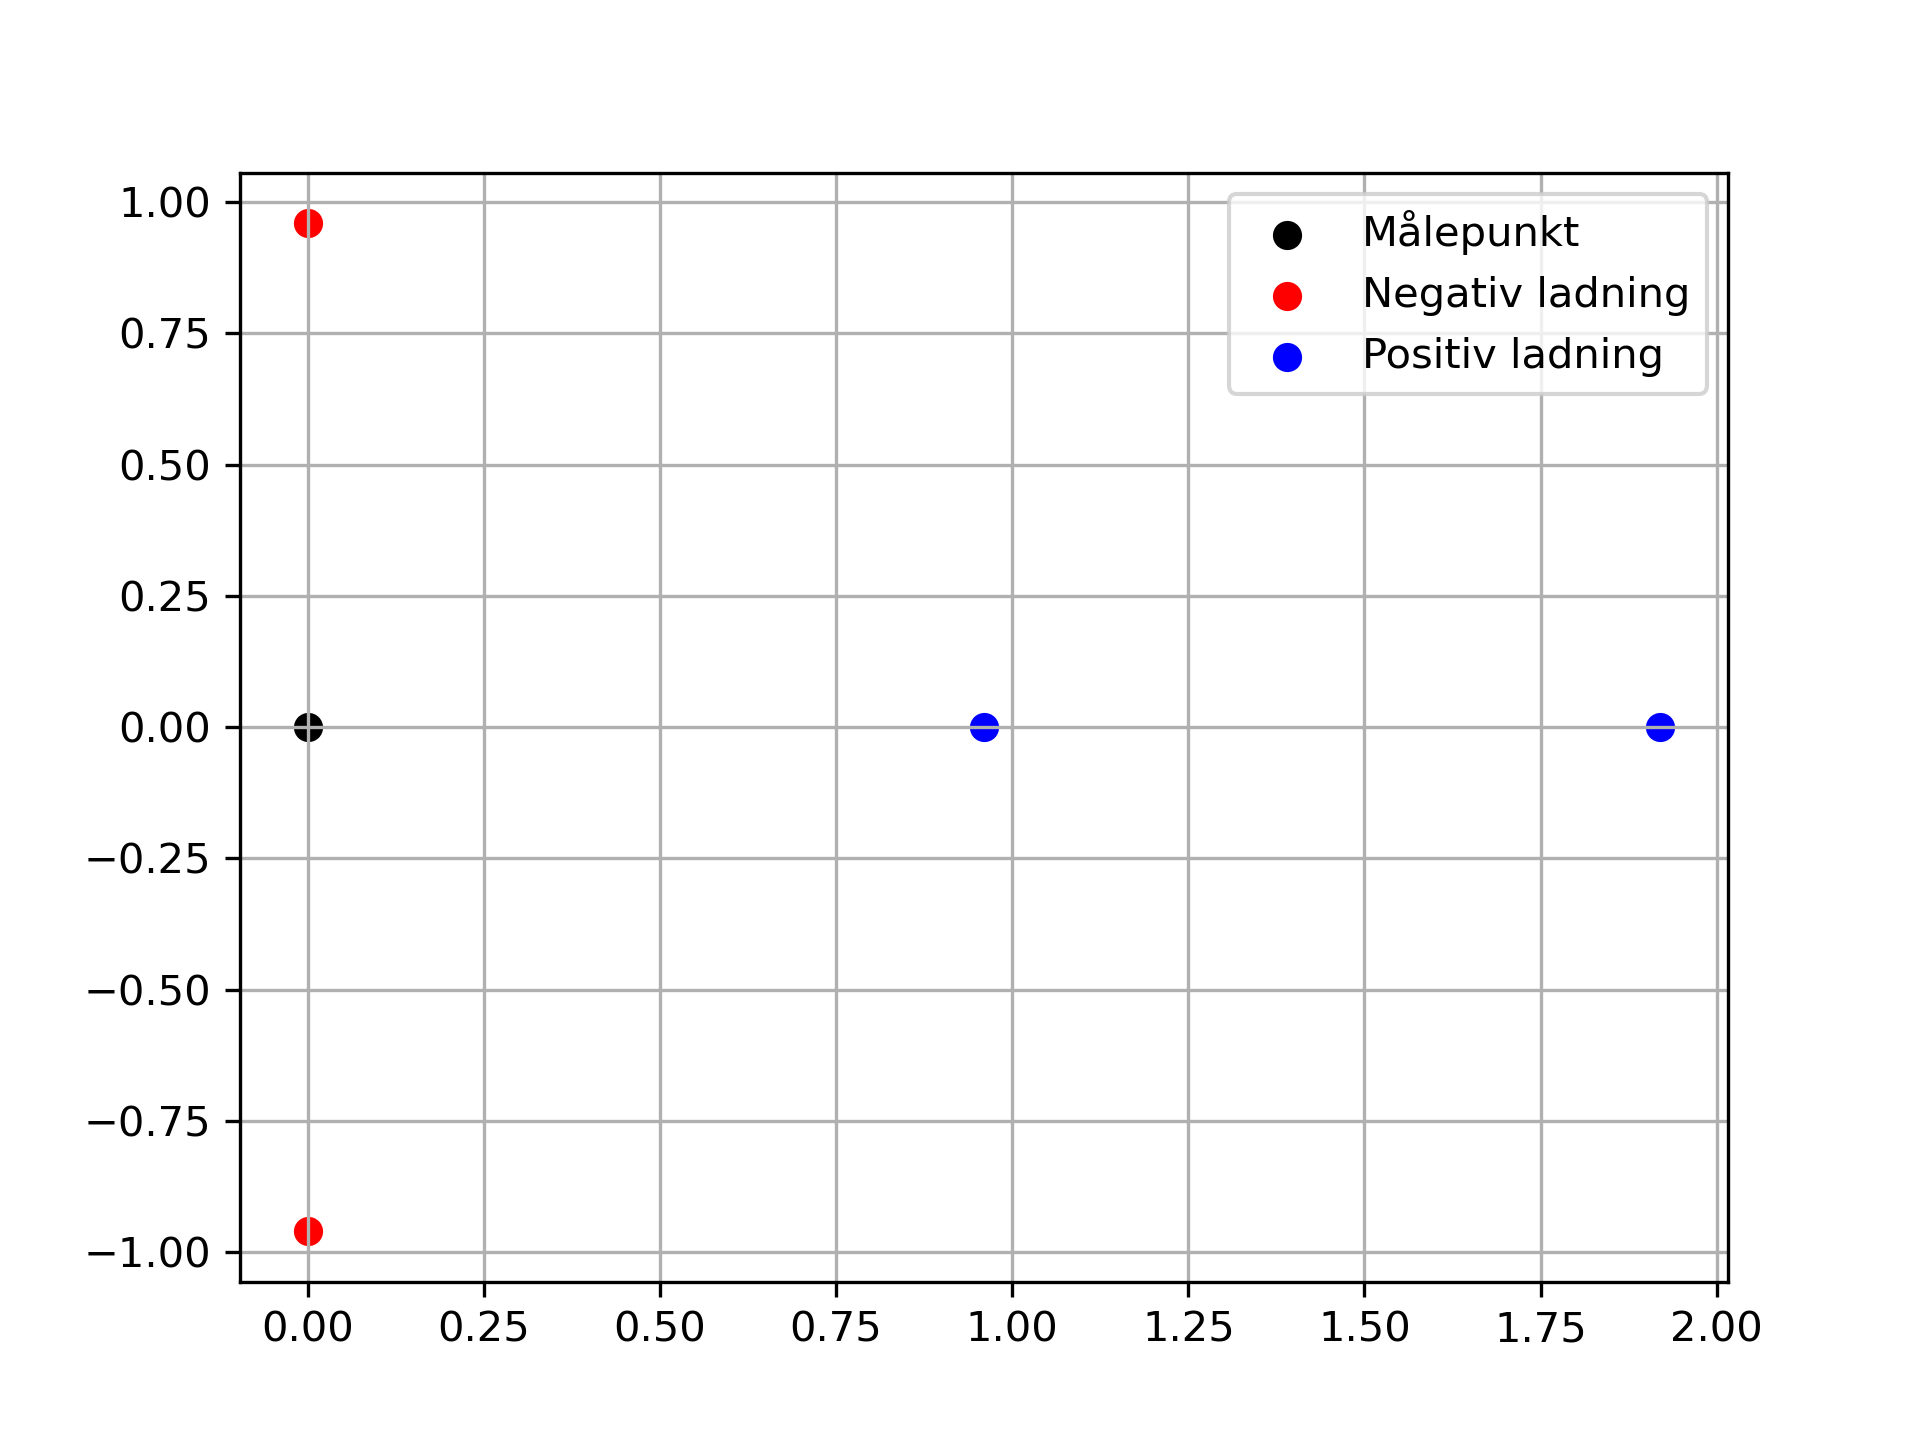
\includegraphics[width=\textwidth]{../oppgave_bilder/Oppgave19_17.png}
\end{minipage}

Elektrisk potensial er gitt ved summen av komponentpotensialene:

$$V_P = \frac{1}{4\pi\epsilon_0}\sum_{i=1}^{N}{\frac{q_i}{r}} $$

$$V_P = \frac{1}{4\pi\epsilon_0}\left(\frac{-q}{d} + \frac{-q}{d} + \frac{q}{d} + \frac{q}{2d}\right)$$

Setter inn verdier

$$V_P = \frac{1}{4\pi\epsilon_0}
\left(
\frac{-2.0\mu, \mathrm{C}}{0.96\, \mathrm{m}} + 
\frac{-2.0\mu, \mathrm{C}}{0.96\, \mathrm{m}} +
\frac{2.0\mu, \mathrm{C}}{0.96\, \mathrm{m}} +
\frac{2.0\mu, \mathrm{C}}{1.92\, \mathrm{m}}
\right)$$

\centerline{\underline{\underline{$V_P = -9.4 \times 10^{3}\, \mathrm{V}$}}}

\newpage
\section*{Oppgave 26}

\begin{minipage}{0.45\textwidth}
  % Your text goes here on the left side.

Konstanter:

$$d = 0.40\, \mathrm{m}$$
$$q = 2.0 \mu \, \mathrm{C}$$

\end{minipage}%
\begin{minipage}{0.55\textwidth}
  % Your image goes here on the right side.
  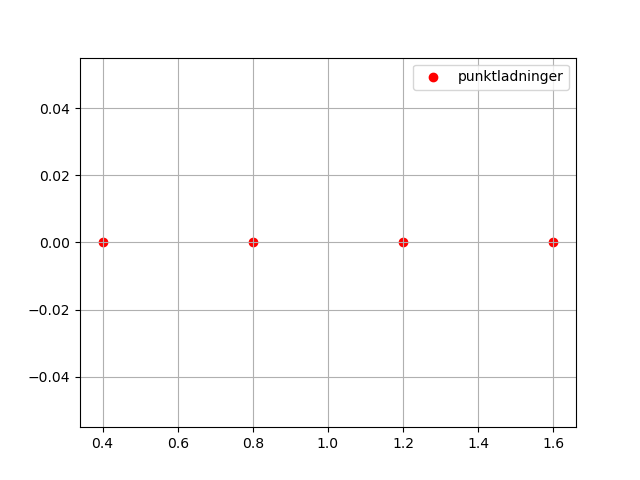
\includegraphics[width=\textwidth]{../oppgave_bilder/Oppgave19_26.png}
\end{minipage}

\newpage
\section*{Oppgave 41}


\newpage
\section*{Oppgave 51}


\newpage
\section*{Oppgave: radioaktivitet}

\end{document}